%!TEX root = ms.tex

\section{Cheeger-Buser inequalities require carefully chosen $\alpha, \beta,
\gamma$}
\label{sec:examples}

% In this section, we consider two  different density functions $\rho$ on the real line.
% One for which Buser direction fails and the other for which Cheeger direction fails. We begin with the Buser direction.

In this section, we prove Lemma~\ref{lem:cheeger-converse} and
Lemma~\ref{lem:buser-converse}. As a consequence, we show that
settings of $\alpha, \beta, \gamma$ common in past work (see
Section~\ref{sec:past-prob}) violates either the Cheeger or Buser
inequality.

We consider two simple density functions:
\begin{enumerate} 
  \item The function $\rho_1(x) = \epsilon/2$ for $-\frac{1}{\epsilon}
    < x < \frac{1}{\epsilon}$, with a $1$-Lipschitz dropoff to $0$
    at the endpoints of $[-\frac{1}{\epsilon},
    \frac{1}{\epsilon}]$.
  \item The function $\rho_2(x) = \min(|x|+\epsilon,
    -|x|+\sqrt{2})$ for $|x| < \sqrt{2}$ and $\rho_2(x) = 0$
    for $|x| > \sqrt{2}$.
\end{enumerate}

\begin{figure}[H]
\centering
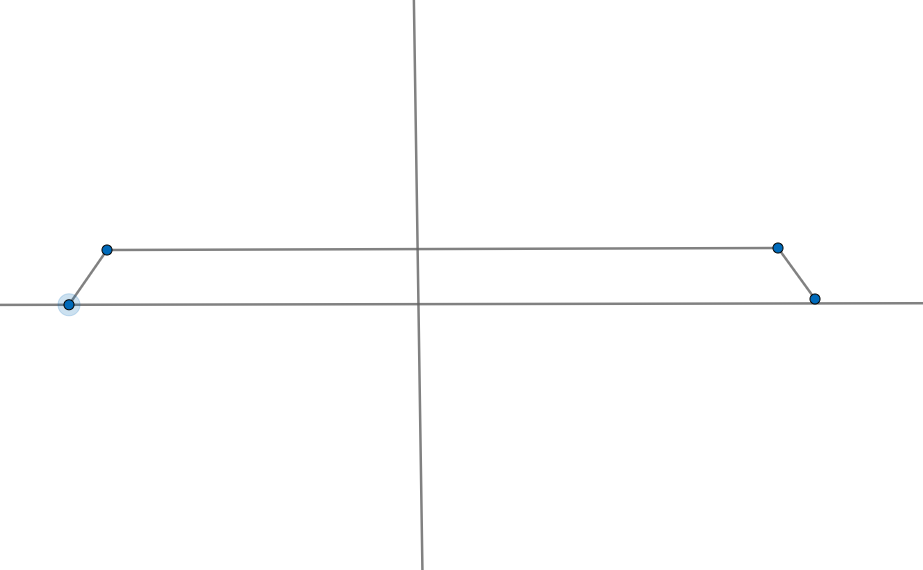
\includegraphics[width=2.5in]{spectralcluster/images/cheeger-counterexample.png}
\caption{
  The function $\rho_1$, a $1$-Lipschitz counterexample to Cheeger's inequality
  when $\alpha + \gamma > 2\beta$. 
  The height of the
  function is $\epsilon/2$, and the length of the supporting
  interval is roughly $\frac{2}{\epsilon}$.
 }
\label{fig:buser-counterexample}
\end{figure}

\begin{figure}[H]
\centering
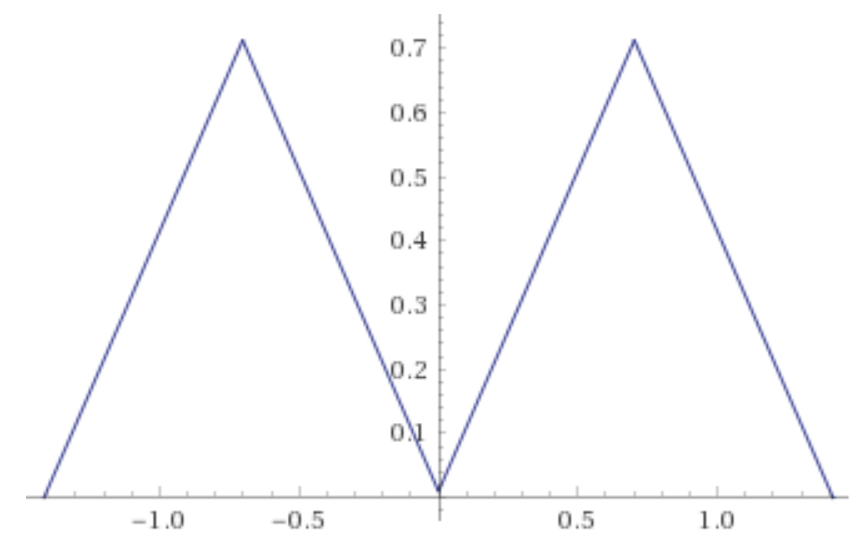
\includegraphics[width=2.5in]{spectralcluster/images/buser-counterexample.png}
\caption{
  The function $\rho_2$, a $1$-Lispchitz counterexample to Buser's inequality
  when $\gamma \geq 1$ and $ \gamma - 1 < \beta$.
 }
\label{fig:buser-counterexample}
\end{figure}


We will show that if $\alpha, \beta, \gamma$ satisfy $\alpha +
\gamma > 2\beta$, then the Cheeger inequality will fail for
$\rho_1$, and if $\gamma \geq 1$ and $\gamma - 1 < \beta$, then the Buser inequality
will fail for $\rho_2$.

In example $\rho_1$, let $\epsilon < 0.01$. The $(\alpha, \beta)$ isoperimetric constant
$\Phi$ is $O((1/\epsilon)^{\alpha - \beta - 1})$, and the eigenvalue
is $O((1/\epsilon)^{\alpha - \gamma - 2})$.  Therefore, the Cheeger
inequality will fail for some $\epsilon$ if $2 (\alpha - \beta - 1) > \alpha - \gamma -
2$, or $\alpha + \gamma > 2\beta$. This proves
Lemma~\ref{lem:cheeger-converse}.

In example $\rho_2$, let $\epsilon < 0.01$. The $(\alpha, \beta)$ isoperimetric constant
$\Phi$ is $O(\epsilon^{\beta})$. The eigenvalue
$\lambda_2$ is lower bounded by $O(\epsilon^{\gamma-1})$ when
$\gamma > 1$, and $\ln(1/\epsilon)$ when $\gamma =1$.
In either case, the Buser inequality will fail if $\gamma - 1 <
\beta$, proving Lemma~\ref{lem:buser-converse}.

We show details of our eigenvalue and isoperimetry calculations
in Appendix~\ref{app:examples}.

